\section{Report Elements}
\label{sec:api_report_elements}

Since characteristics use report elements, we introduce report elements first.
Report elements were introduced in chapter \ref{chapter:xbrl}.
There are multiple types of report elements, which are all represented by different classes in Brel.
All of these classes implement a common interface called \texttt{IReportElement}.

In total, we introduced six different types of report elements:

\begin{enumerate}
    \item \textbf{Concept} - Concepts define what kind of information a fact represents.
    \item \textbf{Abstract} - Abstracts are used for grouping other report elements.
    \item \textbf{Dimension} - Dimensions are used to describe a custom axis, along which a fact is positioned. 
    \item \textbf{Member} - Members specify the point along a dimension that a fact is positioned at.
    \item \textbf{LineItems} - Line items are used to group concepts into an axis, 
    similar to how dimensions group members into an axis.
    \item \textbf{Hypercube} - Hypercube elements describe a smaller sub-hypercube of the filing's global hypercube.
\end{enumerate}

Technically, only concepts, members and dimensions are part of the OIM, whereas the remaining three are not.
However, from an editorial point of view, it makes sense to describe all of them in one place.
Brel chooses to implement report elements as seen in figure \ref{fig:brel_report_element_classes}.

\begin{figure}[H]
    \centering
    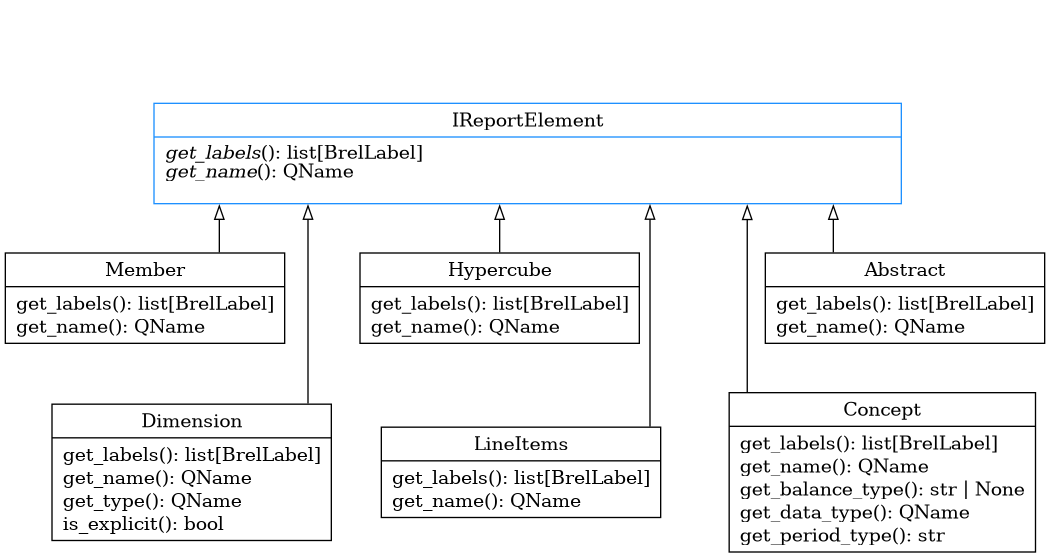
\includegraphics[width=\textwidth]{images/brel_report_elements_classes.png}
    \caption{UML diagram of the report element classes in Brel}
    \label{fig:brel_report_element_classes}
\end{figure}

As a general rule of thumb, we designed Brel's inheritance hierarchy to be as flat as possible.
Since all report elements share a common interface, the next section covers the interface first.
The subsequent sections then describe the different types of report elements.

\subsection{IReportElement}

The \texttt{IReportElement} interface defines the common interface that all report elements share.
In essence, a report element is nothing more than an name, in this case a QName.
QNames were introduced in chapter \ref{chapter:xbrl} and their class was described in section \ref{subsec:qname}.
Since QNames are not completely human-readable and do not support multiple languages,
Brel also provides a method for getting the label of a report element.
This chapter has not yet covered labels, but they will be described in section \ref{sec:labelLink}.
However, they should be conceptually self-explanatory.

The \texttt{IReportElement} interface provides the methods \texttt{get\_qname} and \texttt{get\_labels}, 
which act as their names suggest.
The \texttt{get\_labels} method returns a list of labels, since a report element can have multiple labels.

\subsection{Concept}

The \texttt{Concept} is the most important report element in XBRL.
Concepts are the type of report element that are required to be present in every fact.
They define what kind of information a fact represents.

Besides the methods that are inherited from the \texttt{IReportElement} interface,
the \texttt{Concept} also provides information about its associated facts.

TODO: finish this section

\subsection{Dimension}

Dimensions are used to describe a custom axis, along which a fact is positioned.
Dimensions come in two different flavors, explicit and typed.
Besides the methods that are inherited from the \texttt{IReportElement} interface,
the \texttt{Dimension} has two additional methods.
The first method \texttt{is\_explicit} returns a boolean value, indicating whether the dimension is explicit or not.
The second method \texttt{get\_type} returns the type of the dimension, if it is typed.
It raises an exception if the dimension is explicit.

There is no need for the method \texttt{get\_members} in the \texttt{Dimension} class,
since Brel models members differently.
The dimension-member relationship is modeled as a parent-child relationship between the \texttt{Dimension} and \texttt{Member} objects in definition networks.
So the members of a dimension change depending on the component that the dimension is part of.

We chose to combine both typed and explicit dimensions into a single class,
since they are semantically very similar.
They occupy the same position within networks, but have some slight differences in their behavior.
From a user's perspective, these differences are negligible.

\subsection{Abstract, Hypercube, LineItems, and Member}

% The \texttt{Abstract}, \texttt{Hypercube} and \texttt{Member} classes are all very similar.
The \texttt{Abstract}, \texttt{Hypercube}, \texttt{LineItems} and \texttt{Member} classes are all very similar.
Essentially, their only differentiating factor is their name.
Besides that, they all provide the same methods and attributes.
Namely, they implement the \texttt{IReportElement} interface.
We decided to split them into four different classes, since they are semantically different.
